\documentclass{article}
\usepackage[english]{babel}
\usepackage[utf8]{inputenc}
\usepackage{fancyhdr}
\usepackage[top=2cm, bottom=4.5cm, left=2.5cm, right=2.5cm]{geometry}
\usepackage{graphicx}
\usepackage{amsmath}
\usepackage{amsfonts}
\usepackage{hyperref}
\usepackage{enumerate}
\usepackage{xcolor}


\setlength\parindent{0pt}

% Edit these as appropriate
\newcommand\course{CS 1420}
\newcommand\semester{Fall 2026}            % <-- current semester
\newcommand\hwnumber{7}                      % <-- homework number
\newcommand\duedate{Thursday, November 12, 2026 at 12:00pm \textbf{(Noon)}}

\begin{document}
   \begin{center}
      \huge\textbf{Homework \hwnumber}
   \end{center}

   \begin{center}
        \large{Due: \duedate}
   \end{center}
\section*{\LARGE Written Assignment}
\subsection*{Problem 1: K-Nearest Neighbors and Fairness}
(20 points)

\bigskip
A company uses a classifier to decide whether to invite applicants
for an interview. Each applicant is represented by two numerical
features, $x_1$ and $x_2$, and belongs to one of two groups:
$S=1$ (protected group) or $S=0$ (privileged group).
The group membership $S$ is \textbf{not} used as a feature
by the classifier.

The training set is:

\[
\begin{array}{c|c|c|c}
\text{Applicant} & (x_1,x_2) & S & Y\\
\hline
1 & (1,0)   & 1 & 0\\
2 & (0.5,2) & 1 & 0\\
3 & (0,1.5) & 1 & 1\\
4 & (2.5,1) & 0 & 1\\
5 & (4,0)   & 0 & 1\\
6 & (5,3)   & 0 & 0
\end{array}
\]

Here, $Y=1$ indicates an applicant who would be successful
in the job, while $Y=0$ indicates an applicant who would not.
The company trains a $K$-nearest-neighbors (KNN) classifier
using Euclidean distance. A positive prediction $\hat{Y}=1$
means that the applicant is invited for an interview.

\begin{enumerate}

\item[(a)] Consider the test applicant $x=(2,1)$.

Compute the prediction $\hat{Y}$ for $K=1$, $K=3$, and $K=5$.
Show the relevant distances and identify the neighbors used
for each prediction.

\textbf{Solution:} Use Euclidean distance to calculate the distance between the test applicant $x=(2,1)$ and each training example:

\[
\begin{aligned}
d(x,x_1)
&=\sqrt{(2-1)^2+(1-0)^2}
=\sqrt{2}\approx1.414,\\
d(x,x_2)
&=\sqrt{(2-0.5)^2+(1-2)^2}
=\sqrt{3.25}\approx1.803,\\
d(x,x_3)
&=\sqrt{(2-0)^2+(1-1.5)^2}
=\sqrt{4.25}\approx2.062,\\
d(x,x_4)
&=\sqrt{(2-2.5)^2+(1-1)^2}
=0.5,\\
d(x,x_5)
&=\sqrt{(2-4)^2+(1-0)^2}
=\sqrt{5}\approx2.236,\\
d(x,x_6)
&=\sqrt{(2-5)^2+(1-3)^2}
=\sqrt{13}\approx3.606.
\end{aligned}
\]

Then we sort the applicants from the closest distance to the furthest distance: $4,\;1,\;2,\;3,\;5,\;6$ with the corresponding labels $1,\;0,\;0,\;1,\;1,\;0$.

For $K=1$, the nearest neighbor is applicant 4 with label $Y=1$. Therefore,
$\hat{Y}_{K=1}=1$.

For $K=3$, the 3 nearest neighbors are applicants 4, 1, and 2 with labels $(1,0,0)$. Since the majority label is 0, $\hat{Y}_{K=3}=0$.

For $K=5$, the 5 nearest neighbors are applicants 4, 1,
2, 3, and 5, with labels $(1,0,0,1,1)$. Since the majority label is 1, $\hat{Y}_{K=5}=1$.


\item[(b)] Explain how increasing $K$ generally affects
the complexity of the decision boundary, the training error,
and the tendency of the classifier to overfit.

\textbf{Solution:} Increasing $K$ will generally give a smoother and
less complex decision boundary because predictions depend on more neighborhoods rather than individual training examples.

Training error generally increases as $K$ increases, but it is not necessarily monotonic for every value of $K$. Smaller $K$ will make the classifier sensitive to individual noise, increasing the risk of overfitting. Thus a larger $K$ reduce the risk of overfitting but a too large $K$ will likely cause underfitting.

\item[(c)] The company evaluates its classifier on a separate
test set and obtains the following results:

\[
\begin{array}{l|cc}
 & S=1 & S=0\\
\hline
\text{Number of applicants} & 100 & 100\\
\text{Actually successful }(Y=1) & 50 & 25\\
\text{Predicted positive }(\hat{Y}=1) & 40 & 40\\
\text{True positives }(Y=1,\hat{Y}=1) & 30 & 20
\end{array}
\]

Compute $P(\hat{Y}=1 \mid S=1)$ and
$P(\hat{Y}=1 \mid S=0)$.

Does the classifier satisfy \textbf{statistical parity}?
Does it satisfy the \textbf{80\% rule} for disparate impact?
Justify your answers.

\textbf{Solution:} 

$P(\hat{Y}=1\mid S=1)=\frac{40}{100}=0.4$

$P(\hat{Y}=1 \mid S=0)=\frac{40}{100}=0.4$

Since both groups have the same positive prediction rate, statistical parity is satisfied.

$DI = \frac{P(\hat{Y}=1\mid S=1)}{P(\hat{Y}=1\mid S=0)} = \frac{0.4}{0.4}=1.$

Since $1\geq0.8$, the classifier also satisfies the 80\% rule.


\item[(d)] Compute
\[
P(\hat{Y}=1 \mid Y=1,S=1)
\quad \text{and} \quad
P(\hat{Y}=1 \mid Y=1,S=0).
\]

Does the classifier satisfy the \textbf{positive-rate parity}
condition discussed in class?

\textbf{Solution:}

$P(\hat{Y}=1 \mid Y=1,S=1)=\frac{30}{50}=0.6$

$P(\hat{Y}=1 \mid Y=1,S=1)=\frac{20}{25}=0.8$

Since the true positive rates aren't equal across groups ($0.6\neq0.8$), positive-rate parity is not satisfied.

\item[(e)] Compute
\[
P(Y=1 \mid \hat{Y}=1,S=1)
\quad \text{and} \quad
P(Y=1 \mid \hat{Y}=1,S=0).
\]

Does the classifier satisfy \textbf{predictive rate parity}?

\textbf{Solution:}

$P(Y=1 \mid \hat{Y}=1,S=1)=\frac{30}{40}=0.75$

$P(Y=1 \mid \hat{Y}=1,S=0)=\frac{20}{40}=0.5$

Since the positive predictive values aren't equal across groups ($0.75\neq0.5$), predictive rate parity is not satisfied.

\item[(f)] The company claims that its classifier is fair because
it does not use the protected attribute $S$ and satisfies
statistical parity.

Explain briefly why this conclusion is not necessarily justified.
In your answer, refer to the fairness metrics computed above
and discuss why excluding protected attributes from training
does not guarantee fairness.

\textbf{Solution:} No. Excluding the protected attribute $S$ does not necessarily guarantee fairness because there might exist other features having correlated with membership and thus acting as proxy variables. In the case above, the classifier satisfies statistical parity and the 80\% rule, but fails both positive-rate parity and predictive rate parity. Therefore, statistical parity alone and the exclusion of protected attributes are insufficient to establish that the classifier is fair under all relevant fairness criteria.

\end{enumerate}
\newpage
\subsection*{Problem 2: Principal Component Analysis}
(20 points)

\bigskip
In this question, you will build a spam filter using Principal Component Analysis (PCA) and the K-Nearest Neighbour algorithm.

\medskip
The K-Nearest Neighbour algorithm is a simple-to-implement classifier in which an example is labeled with the most common label among the K closest examples in the training data.
(Ties can be broken randomly.)
Here, ``closest'' refers to Euclidean distance.

\medskip

You will be using PCA to transform the e-mail data from 2 dimensions (and a label) to 1 dimension (and a label). Each e-mail has two features: number of words in the email and total occurrences of the spam words ``credit'' and ``dollars''. The following graph shows the training data where filled circles are spam e-mails and unfilled circles are non-spam emails. The x-axis (Total words count) has been scaled for your convenience.

\medskip
We have found the first principal component: $(\frac{1}{\sqrt{2}},\frac{1}{\sqrt{2}})$.
Therefore the linear subspace that PCA will project the data to is the line $y = x$.
(Assume that we don't need to do any centering of the data.)

\begin{center}
    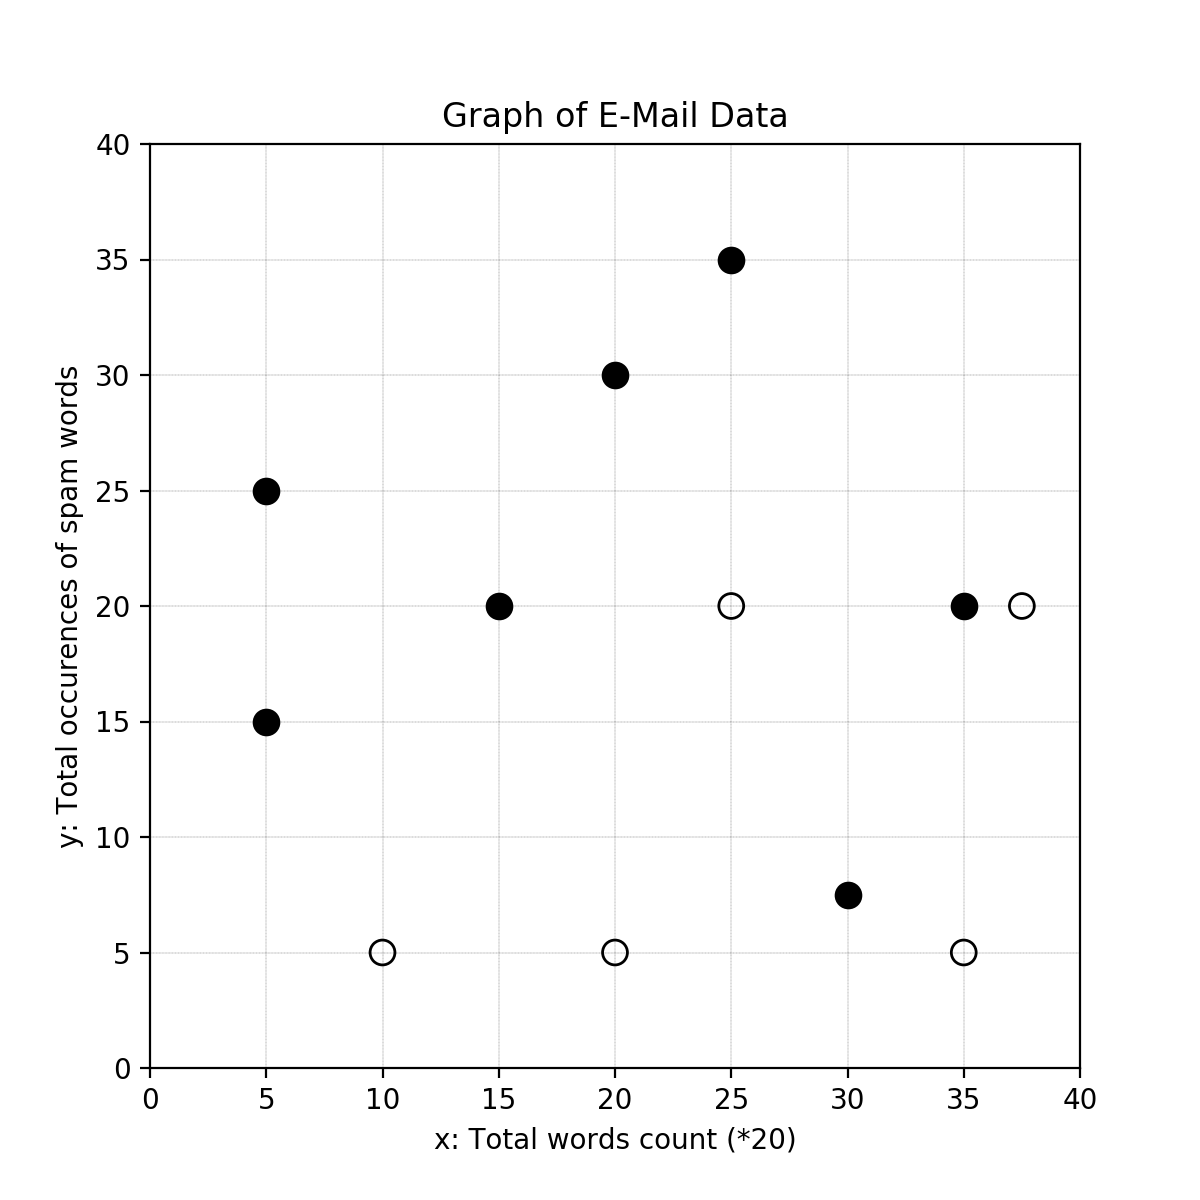
\includegraphics[width=0.5\textwidth]{q1_graph1.png}
\end{center}

\begin{enumerate}[a.]
    \item Draw the first principal component as a line ($y=x$ in this case) on the graph. Also draw the data points projected to this subspace with lines connecting them to the corresponding original data points.

    \textbf{Solution:}

    \begin{center}
    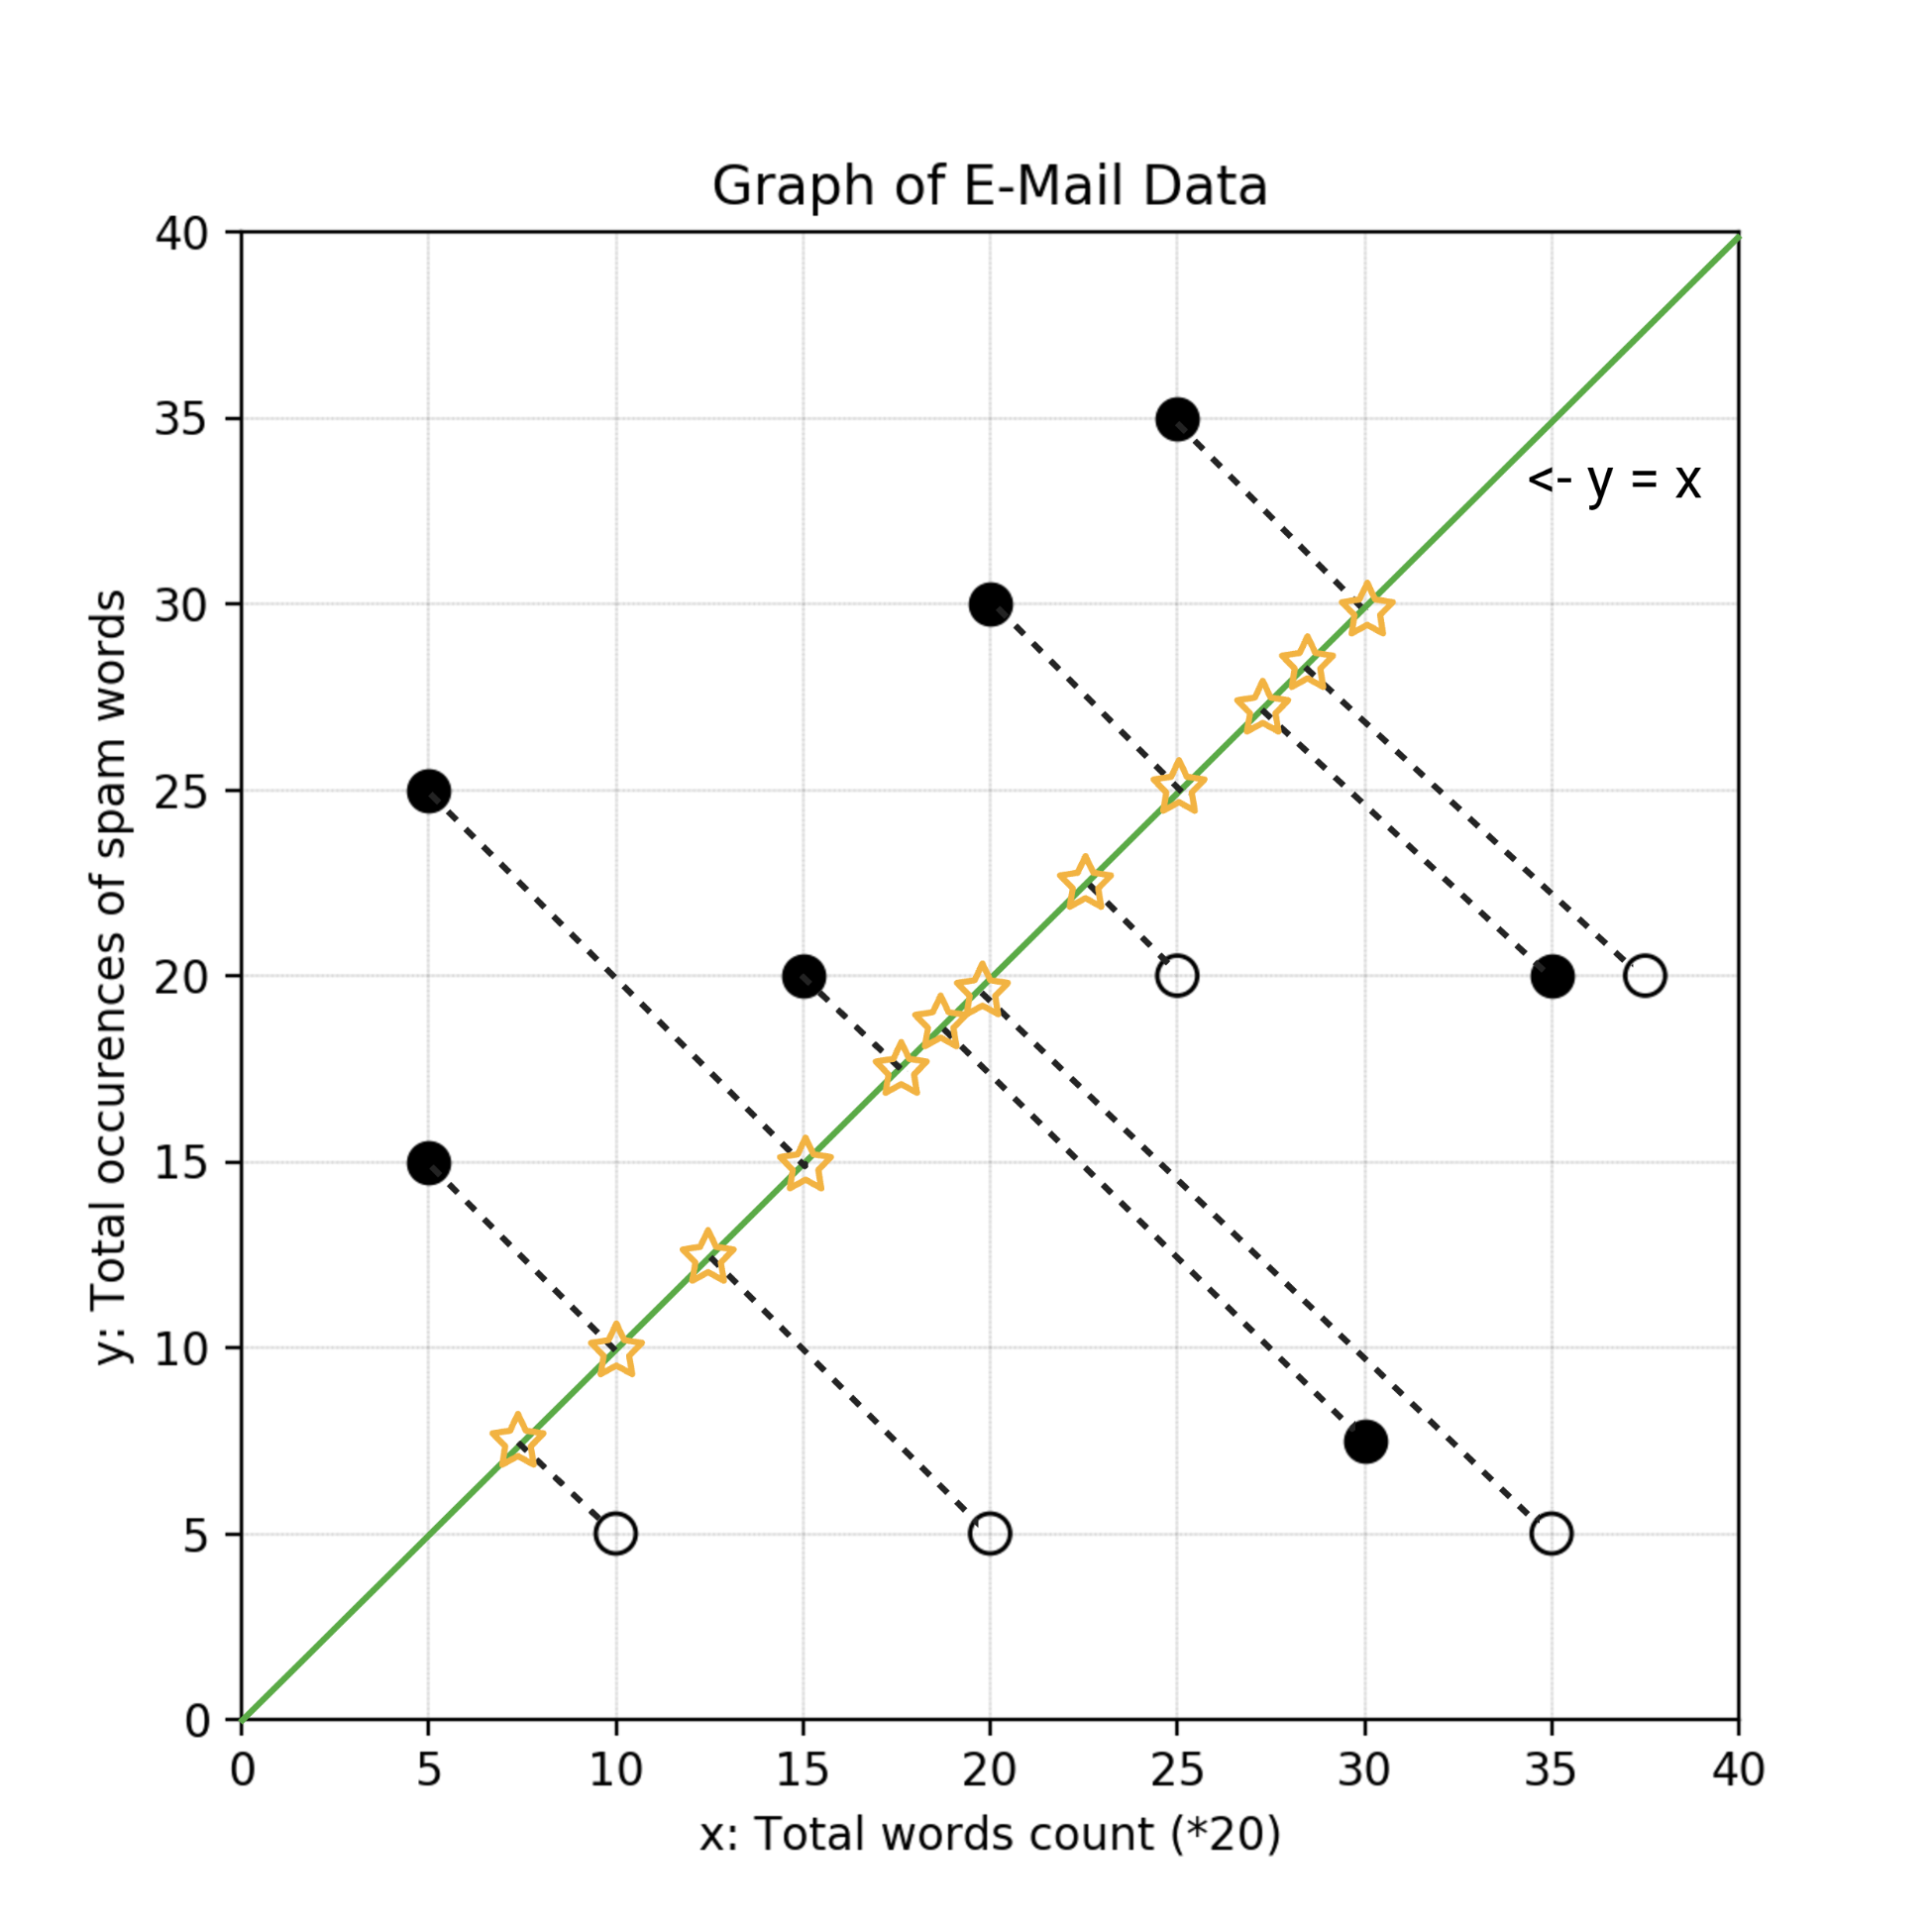
\includegraphics[width=0.5\textwidth]{Part2-a.png}
    \end{center}

    
    \item How would \textbf{1}-Nearest Neighbour algorithm classify an e-mail with 21 spam words in a total of 100 ($x$=5) words? Explain your answer.

    \textbf{Solution:} The test email containing 21 occurrences of spam words and 100 total words has the feature vector $x_{\text{test}}=(5,21)$, since the x-axis is scaled by 20.

    Using Euclidean distance (also can tell from the graph), the closest training example is the spam email at $(5,25)$, with the Euclidean distance from the test email as

    \[
    d((5,21),(5,25))=\sqrt{(5-5)^2+(21-25)^2}=\sqrt{0+16}=4.
    \]

    Therefore, 1-NN assigns the email as $\hat{Y}_{\text{before PCA}}=\text{Spam}$.
    
    \item How would \textbf{1}-Nearest Neighbour algorithm classify the same e-mail given in the previous question after transforming the data to 1-dimension? Explain your answer.

    \textbf{Solution:} After PCA, the one-dimensional coordinate of a point $x=(x_1,x_2)$ is $z=x\cdot u =\frac{x_1+x_2}{\sqrt{2}}$.

    For the test email $(5,21)$, $z_{\text{test}} =\frac{5+21}{\sqrt{2}} =\frac{26}{\sqrt{2}}$.

    Now, to find the point closest to this test email, we need to find the one that has the closest sum of $x_1$ and $x_2$, which is $x=(20,5)$ with $z_{\text{test}} =\frac{20+5}{\sqrt{2}} =\frac{25}{\sqrt{2}}$. 

    This is non-spam email. Therefore, 1-NN assigns the test emial as $\hat{Y}_{\text{before PCA}}=\text{Non-spam}$.

    
    \item Are your answers same for part b and c? Why or why not?

    \textbf{Solution:} No, because the predictions are different. Before PCA, the 1-NN predicts according to the closest point $(5,25)$ which is a spam. After PCA, the 1-NN predicts according to the closest point $(20,5)$ which is a non-spam. Projecting data from two dimensions to one dimension discards information in the direction orthogonal to the first principal component. As a result, distances between points can change, and the identity of the nearest neighbor can change.

\end{enumerate}

\newpage

\subsection*{Problem 3: Limitations of PCA (20 points)}
Consider the following two-dimensional dataset:

\begin{center}
    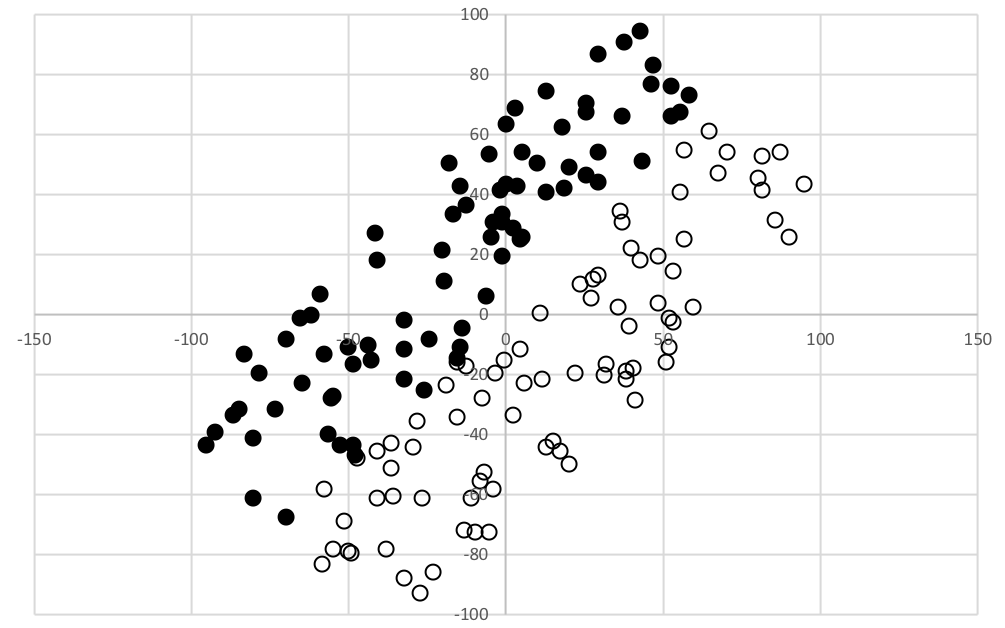
\includegraphics[width=0.8\textwidth]{pca_graph.png}
\end{center}

\begin{enumerate}[a.]
    \item Describe one type of machine learning model that would classify this data well. Explain your reasoning.

    \textbf{Solution:} A linear classifier such as halfspace classifer. Because the black points are generally located above and to the left of the white points. The two classes can be separated approximately by a diagonal decision boundary with positive slope.

    For example, the classifier could be $h(x)=\operatorname{sign}(wx+b)$.

    
    \item Draw the first principal component on the graph above. If PCA was used to reduce this data to one dimension, would the machine learning model from part (a) still classify the data well? Why or why not?

    \textbf{Solution:} The first principal component is approximately the positively sloped diagonal direction from the bottom-left to the top-right of the graph, which captures the greatest variance in the combined dataset.

    If PCA reduces the data from 2D to 2D by projecting onto this principal component, a halfspace classifier would not classify the data as well as it could in the original space, because the two classes are primarily separated in a direction approximately perpendicular to the first principal component.

    Just like what we see in Part2, even although PCA preserves the direction of maximum variance, it may still discard information that is important for classification.

    \begin{center}
    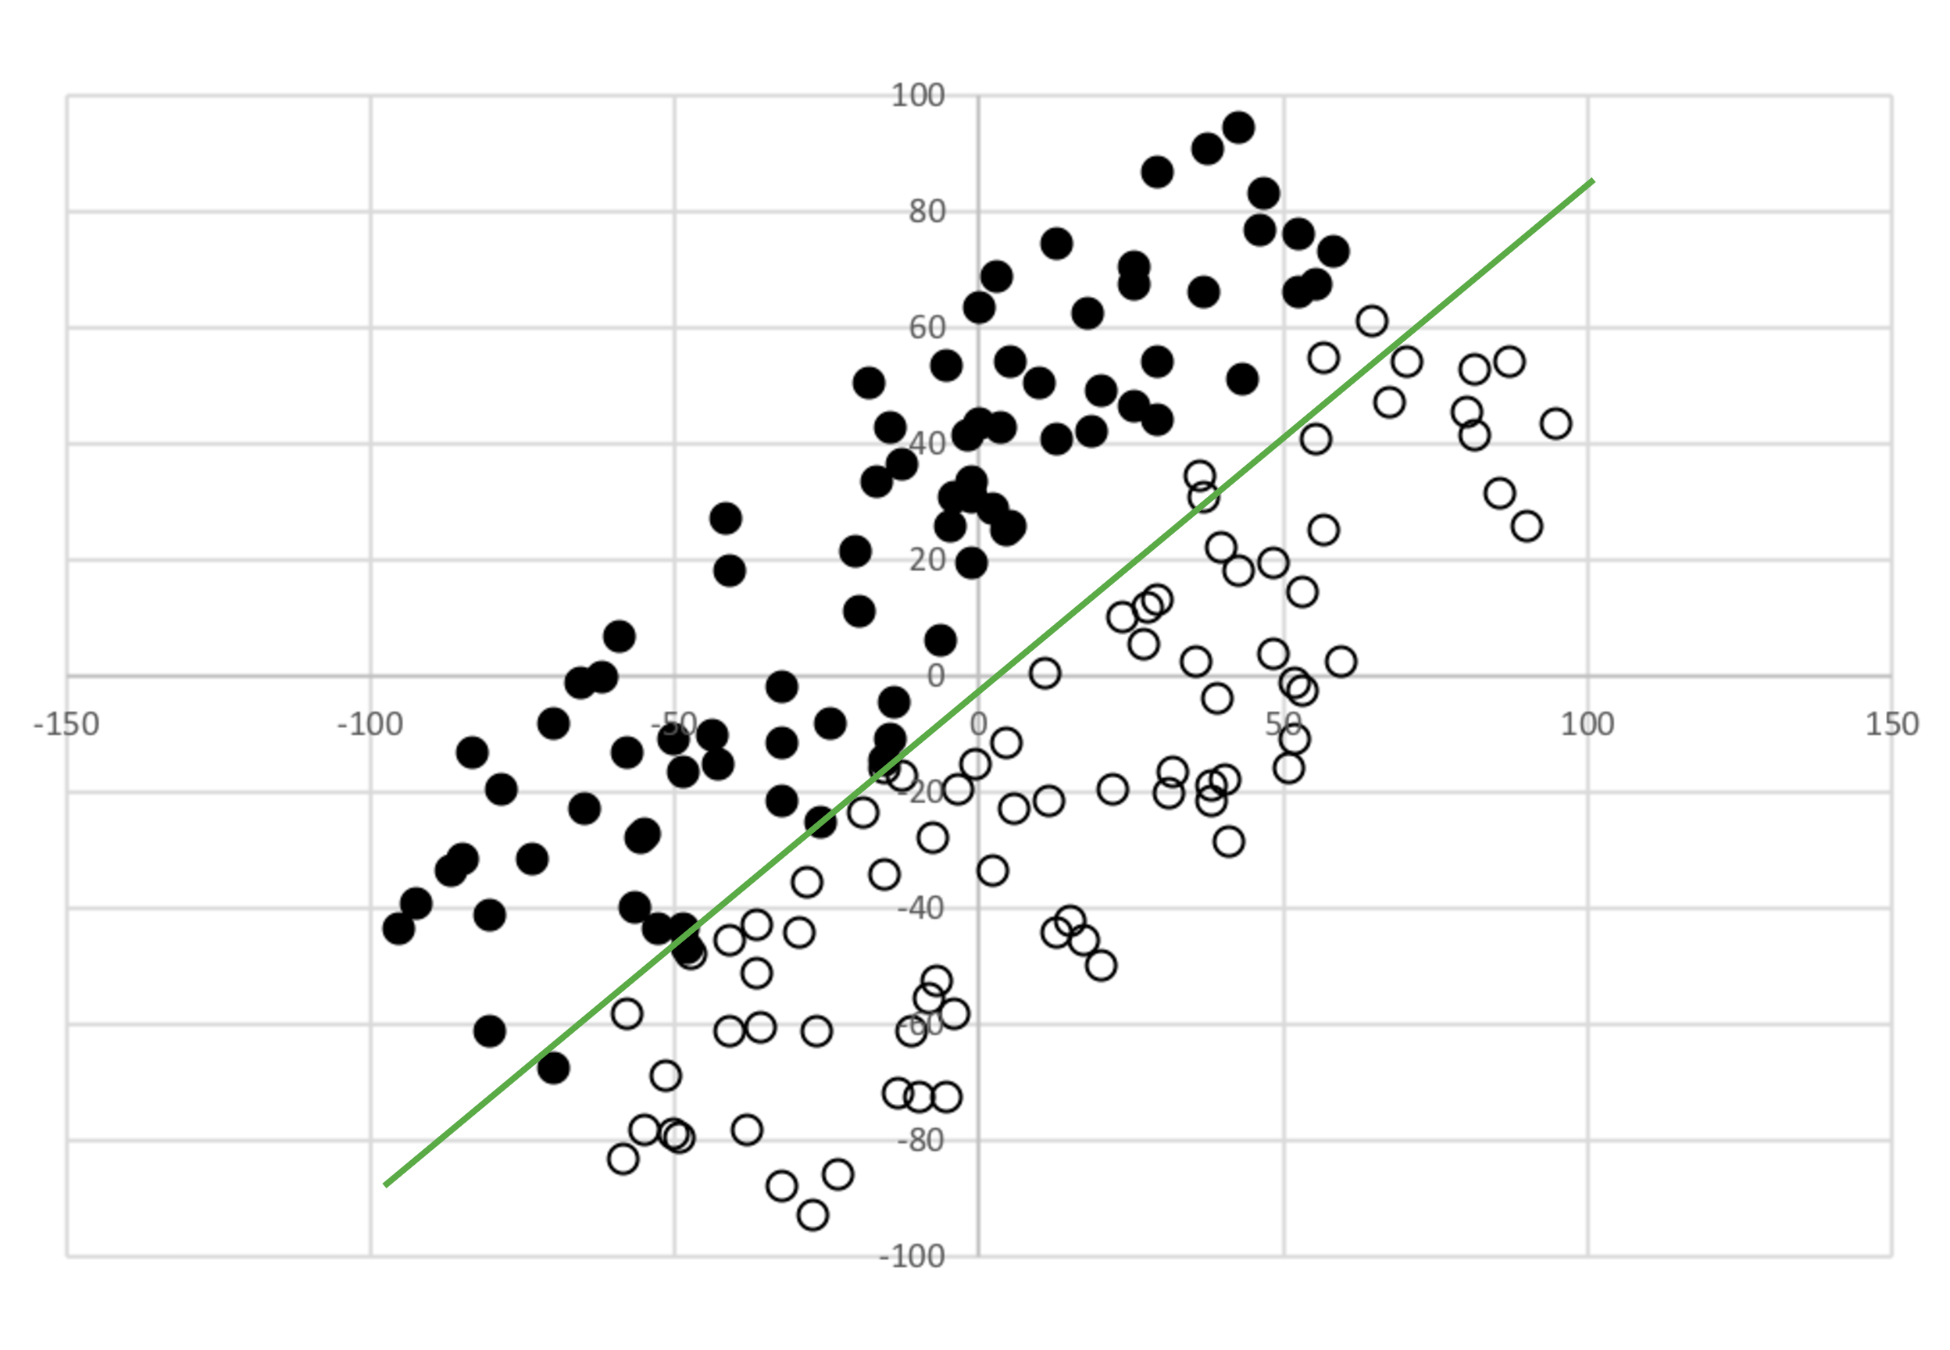
\includegraphics[width=0.8\textwidth]{Part3-b.png}
    \end{center}

    
    \item Is it possible to project the above data into a one-dimensional linear subspace in which the data remains linearly separable? If so, draw the subspace on the graph above. If not, explain your reasoning.

    \textbf{Solution:}

    \begin{center}
    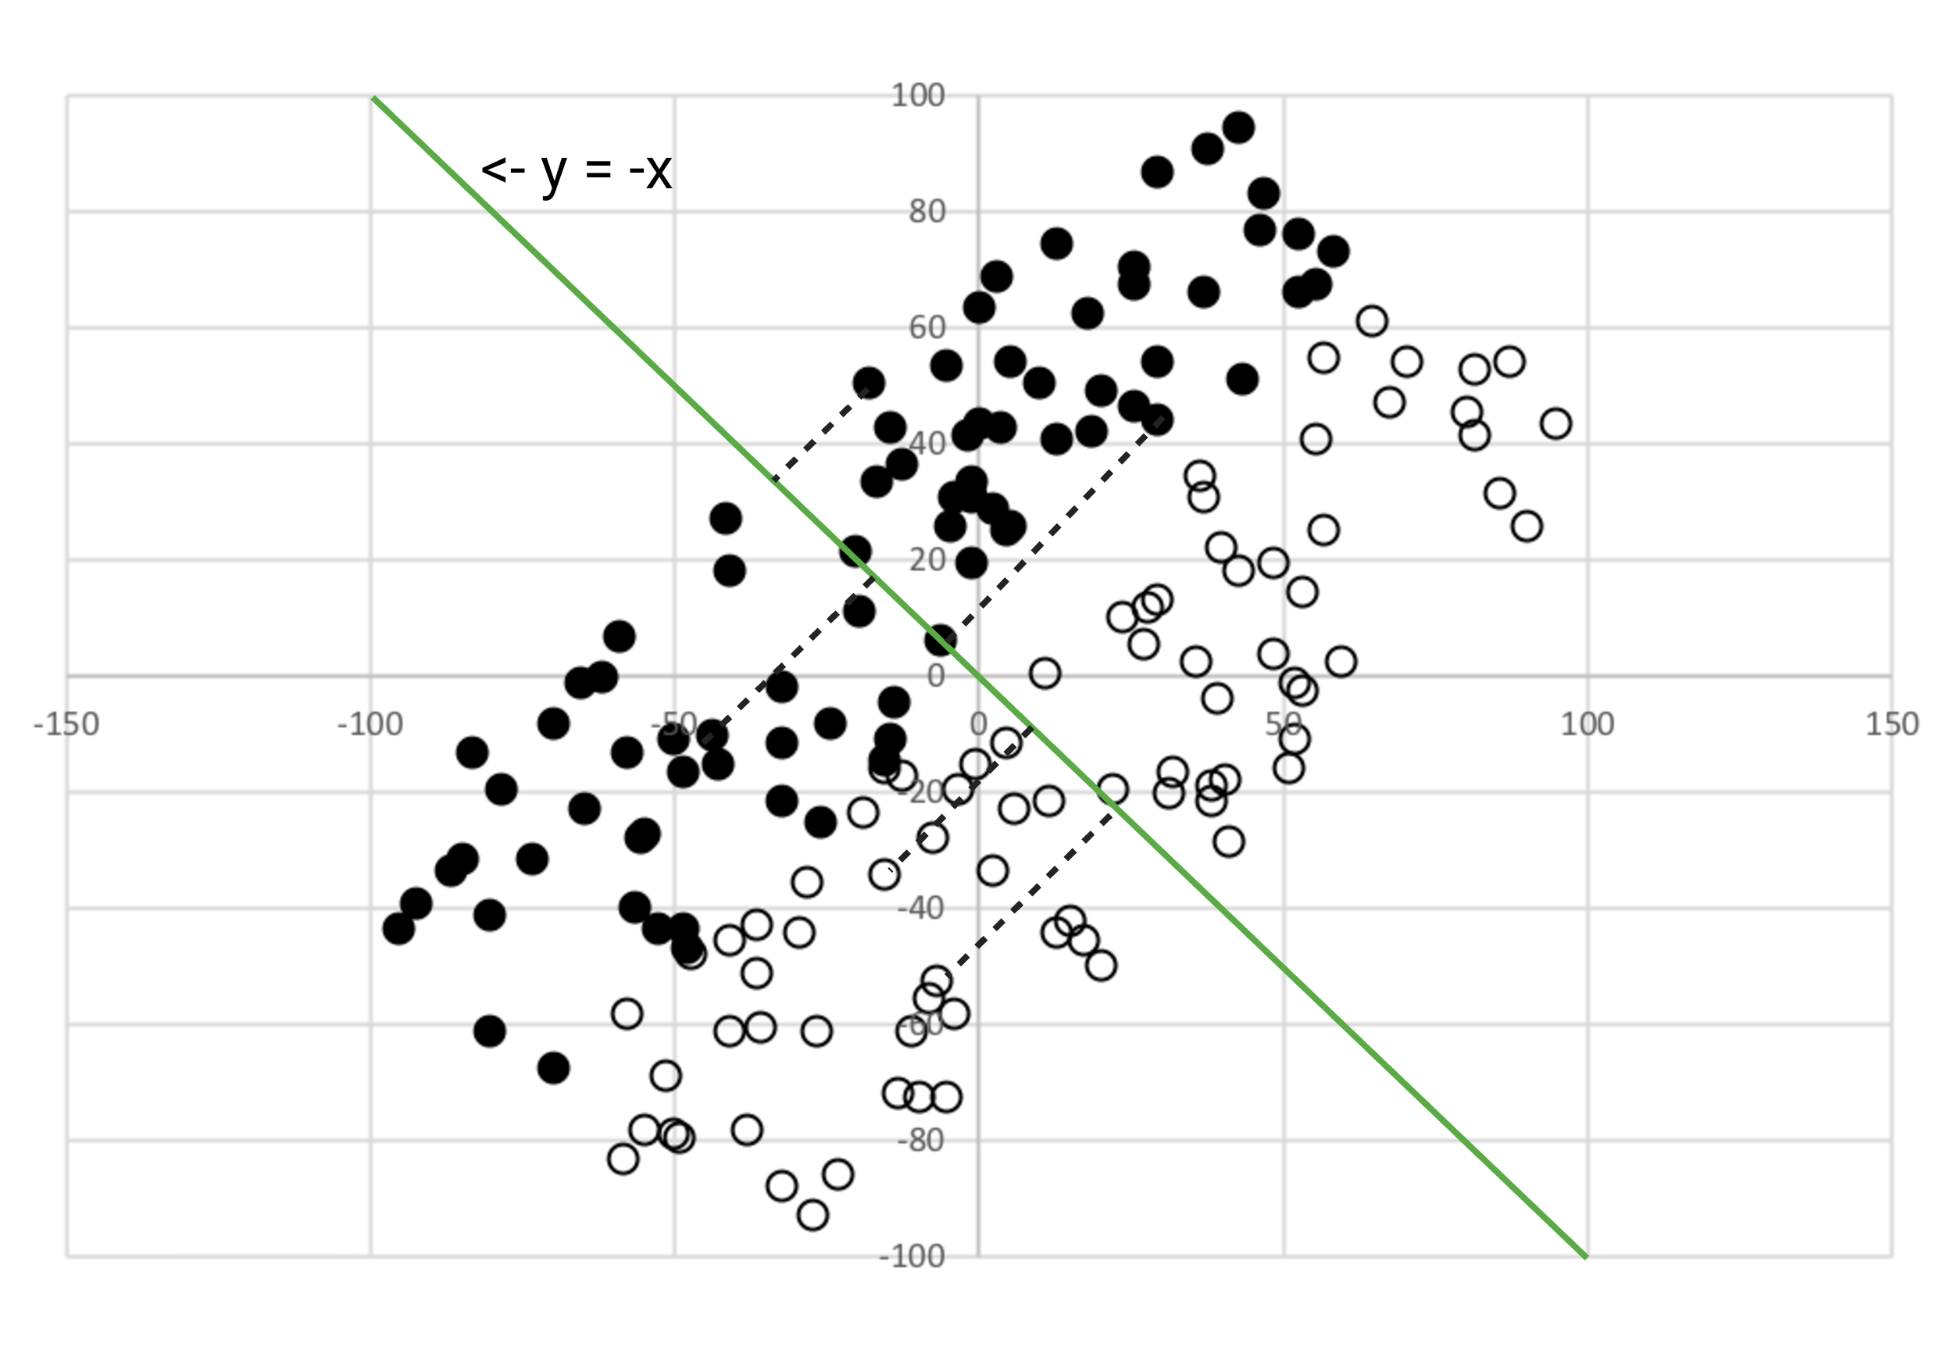
\includegraphics[width=0.8\textwidth]{Part3-c.png}
    \end{center}

    Yes. It's possible that a one-dimensional linear subspace can preserves the separation between the two classes. We can project the data onto a direction approximately perpendicular to the linear decision boundary as shown in the figure $y=x$ or $x_2=-x_1$.

    Since the black points generally lie above and to the left of the white points, they tend to have larger values of $x_2-x_1$, while the white tend to have smaller values. Therefore, the projected values can be approximately separated by a threshold $t$:

    \[
    h(z)=
    \begin{cases}
    1, & z\geq t,\\
    0, & z<t.
    \end{cases}
    \]


    \item What does this example tell you about the limitations of PCA when used to pre-process data before classification?

    \textbf{Solution:} This demonstrates that PCA does not necessarily preserve the information most useful for classification. PCA may reduce classification performance by discarding low-variance directions that contain important class-discriminative information.

\end{enumerate}

\newpage

\section*{\LARGE Programming Assignment}

\subsection*{Introduction}
In this assignment, you'll implement Naive Bayes and use this algorithm to classify the credit rating (good or bad) of a set of individuals. The textbook section relevant to this assignment is 24.2 on page 347.


\subsection*{Stencil Code \& Data}


We have provided the following two files:
\begin{itemize}
	\item \texttt{main.py} is the entry point of your program which will read in the data, run the classifiers and print the results. Note that pre-processing has been done for you; feel free to examine the code for what exactly was done.
	\item \texttt{models.py} contains the \texttt{NaiveBayes} model which you will be implementing.
\end{itemize}

\textbf{You should not modify any code in the \texttt{main.py}}. All the functions you need to fill in reside in \texttt{models.py}, marked by \texttt{TODO}s. You can see a full description of them in the section below. To feed the data into the program successfully, please do \textit{not} rename the data files and also make sure not to move either the data file or \texttt{models.py} from the stencil. To run the program, run \texttt{python main.py} in a terminal.\newline

You can find and download the stencil in the \href{https://drive.google.com/drive/folders/1L2hDZDggpbipDvfng0BQGTFkJgEsLPfM?usp=sharing}{Google Drive folder for Homework 7}. \newline


\subsubsection*{German Credit Dataset}

You will be using the commonly-used German Credit dataset, which includes 1000 total examples. The prediction task is to decide whether someone's credit is good (1) or bad (0). A full list of attributes can be found \href{https://archive.ics.uci.edu/ml/datasets/Statlog+\%28German+Credit+Data\%29}{\textbf{here}}; note that this includes sensitive attributes like sex, age, and personal status. The specific file we are using comes from \href{https://github.com/algofairness/fairness-comparison}{\textbf{Friedler et.al., 2019}}. 
This data is in the file \texttt{german\_numerical-binsensitive.csv}. 

\subsubsection*{Data Format}

The original feature values in this dataset are mixed---some categorical, some numerical. We have written all the preprocessing code for you, transforming numerical attributes into categories and encoding all attributes as binary features. After preprocessing, there are a total of 69 attributes that take on either 1 or 0. \textbf{\texttt{credit = 1} corresponds to ``good" credit, and \texttt{credit = 0} corresponds to ``bad" credit.}


\subsection*{The Assignment}

In \texttt{models.py}, there are three functions you will implement. They are:

\begin{itemize}
\item \texttt{NaiveBayes}:
\begin{itemize}
	\item[\textendash] {\bf train()} uses maximum likelihood estimation to learn the parameters (attribute distributions and prior distribution). Because all the features are binary values, you should use the Bernoulli distribution (as described in lecture) for the features. Apply Laplace smoothing to both the class priors and the conditional attribute distributions. 
	\item[\textendash] {\bf predict()} predicts the labels using the inputs of test data. You should return a 1-D NumPy array.
	\item[\textendash] {\bf accuracy()} computes the fraction of correctly predicted labels over a dataset (a value between 0 and 1).
\end{itemize}
\end{itemize}


You are not allowed to use any off-the-shelf packages that have already implemented Naive Bayes, such as scikit-learn; we're asking you to implement it yourself.
\\\\
\textbf{Note:} Depending on whether or not you assume that the inputs
are given in log-space, the autograder may print out a message
pointing this out. Know that this is not an error message and
should be taken as informational.
\\\\
Note that the \texttt{NaiveBayes} class also includes a {\bf print\_fairness()} method, which has already been implemented for you and should not be modified. This method will be invoked automatically when you run main.py and will report several fairness metrics for your trained classifier, including disparate impact and group-specific false positive and false negative rates. You are not required to analyze these results for this assignment, but you are welcome to explore them if you are interested in evaluating your model's fairness under different criteria.


\subsection*{Project Report}

\begin{enumerate}
    \item Report the training and validation accuracy of the Naive Bayes classifier. (A correct implementation should have validation accuracy above $70\%$.) (2 points)
    
    \item What strong assumption about the features/attributes of the data does Naive Bayes make? Comment on this assumption in the context of credit scores. (6 points)

    
    \item This dataset was originally structured as follows:

    \begin{center}
    \begin{tabular}{| c | c | c | c || c |}
        \hline
    	 Month & Credit Amount & Number of credits & ... & Credit\\
    	\hline
    	6 & 1169 & 2 & ... & 1 \\
    	48 & 5951 & 1 & ... & 2\\
    	12 & 2096 & 1 & ... & 1\\
    	9 & 2134 & 3 & ... & 1 \\
        % 	etc & & & \\ 
    	\hline
    \end{tabular}
    \end{center}
    For each of the above attributes, describe what transformations to the original dataset would need to occur for it to be usable in a Bernoulli Naive Bayes model. \textit{(hint: every attribute must take on the value of 0 or 1)} (10 points)

        
    
    
    
\end{enumerate}


\subsection*{Grading Breakdown}
We expect the accuracy that \texttt{NaiveBayes} reaches should be above 70\%, on both training and validation. Note that your results may fluctuate each time you run the program, as there is some stochasticity in the preprocessing of the data.
As always, you will primarily be graded on the correctness of your code and not based on whether it does or does not achieve the accuracy target. The autograder does not check for the accuracy threshold, but instead checks for correct implementation and prediction results.

The grading breakdown for the assignment is as follows:
\begin{center}
\begin{tabular}{| l | r |}
    \hline
    Written & 60 points\\
	Programming & 60 points \\
	Report & 18 points \\
	\hline
	Total & 138 points \\
	\hline
\end{tabular}
\end{center}


\subsection*{Handing in}
You will hand in both the written assignment and the coding portion on Gradescope, separately. 

\begin{enumerate}
    \item Your written assignment should be uploaded to Gradescope under ``Homework 7". 
    \item Submit your Homework 7 folder containing all your source code and your project report named \textbf{report.pdf} on Gradescope under ``Homework 7 Code". \textbf{report.pdf} should live in the root directory of your code folder; the autograder will check for the existence of this file and inform you if it is not found. For questions, please consult the \href{https://docs.google.com/document/d/1dYim__KVuE9nZj7RBWr9Mw-S6w6EjeFBbSBDxWWWJFA/edit?usp=sharing}{download/submission guide}.
\end{enumerate}


\subsubsection*{Anonymous Grading}
You need to be graded anonymously, so do not write your name anywhere on your hand-in. 


\subsection*{Academic Integrity}
The \href{https://docs.google.com/document/d/1V2w_oecqWRg0Zb9IWdG-5NzGnYnX55G5SG0Pf5jD0N4/edit?usp=sharing}{CSCI 1420 Collaboration Policy} applies to this assignment.
As outlined in the \href{https://college.brown.edu/design-your-education/academic-policies/academic-code}{Brown Academic Code} and the \href{https://graduateschool.brown.edu/academics-research/rules-regulations/academic-code}{Brown Academic Code, Graduate Student Edition}, attempting to pass off another's work or AI-generated work as your own can result in failing the assignment, failing this course, or even dismissal or expulsion from Brown.  More than that, you will be missing out on the goal of your education, which is the cultivation of your own mind, thoughts, and abilities.  Please review this course's collaboration policy and if you have any questions, please contact the instructor.

\end{document}
